\documentclass{../../common/thesisbyxetex}

\usepackage{enumitem}
\setlist{nolistsep}	% отступы между элементами перечесления

\addbibresource{../../common/bibliography.bib}

\usepackage{url}
\usepackage{array}
\usepackage{longtable}
\usepackage{pdflscape}


\renewcommand{\UrlBreaks}{
\do\/\do\a\do\b\do\c\do\d\do\e\do\f\do\g\do\h\do\i\do\j\do\k\do\l\do\m\do\n\do\o\do\p\do\q\do\r\do\s\do\t\do\u\do\v\do\w
\do\x\do\y\do\z\do\A\do\B\do\C\do\D\do\E\do\F\do\G\do\H\do\I\do\J\do\K\do\L\do\M\do\N\do\O\do\P\do\Q\do\R\do\S\do\T\do\U
\do\V\do\W\do\X\do\Y\do\Z}

\begin{document}

\newcolumntype{P}[1]{>{\small\raggedright\arraybackslash}p{#1}}

\hypersetup{
pdftitle = {Контрольная работа, Компьютер в работе психолога},
pdfauthor = {Станкевич Наталия Александровна},
pdfsubject = {контрольная},
pdfkeywords = {компьютер, психология, контрольная}
}% End of hypersetup

\begin{titlepage}
\newpage

\begin{center}
\large \uppercase{Белорусский государственный университет \\
факультет философии и социальных наук\\
кафедра психологии}
\end{center}
 
\vspace{12em}



\begin{center}
\Large \uppercase{\textbf{Курсовая работа}}
\end{center}

\begin{center}
\textbf{Контрольная работа по дисциплине <<Компьютер в работе психолога>>}
\end{center}

\vspace{11em}
 
\begin{flushright}
%\parbox{0.45\textwidth}{
Выполнила:

\vspace{0.25em}

студентка 1 курса отделения психологии

\textbf{Станкевич Наталия Александровна}

\vspace{2em}

Проверила:

\vspace{0.25em}

\textbf{Кулинкович Тамара Олеговна}

%}%end parbox
\end{flushright}

\vspace{2em}
Дата сдачи на кафедру:\underline{~~~~~~~~~~~~~~~~~}
\vspace{0.25em}

Методист:
 
\vspace{\fill}

\begin{center}
Минск, 2015
\end{center}

\end{titlepage} 

\chapter*{Контрольная работа №1}
\section*{I. \uppercase{Что есть дипломная работа и зачем она} 10 \\
I.1. Зачем пишут диплом и что он такое 10 \\
I.2. Кому адресована эта книга 13 \\
I.3. Чем дипломная работа может пригодиться после университета 15 \\
I.4. Четыре простейших правила 16}
Вопросы:
\begin{enumerate}
\item Описание работы, которую профессор Эко называет дипломом, скорее подходит под белорусское определение
диссертации: объем от 100 до 400 страниц --- это от объема кандидатской до объема, вдвое превосходящего докторскую.
Процедура защиты скорее тоже напоминает защиту диссертации (наличие оппонентов). Как все же это соотносится с написанием
белорусского диплома и будут ли актуальны рекомендации профессора для студентов-дипломников?

\item Чем все же отличается понимание понятия диплома и диссертации в книге Эко, если диссертация – это в том числе и
<<систематизация материала по какому-либо вопросу, придающая единство набору идей...>> (с.12), а в дипломе студент
может <<просто демонстрирует, что сумел критически переработать большую часть существующей литературы (то есть книг и
статей, посвященных теме диплома) и внятно изложить прочитанное, соотнося различные точки зрения...>> (с.12). В чем
радикальное различие между систематизацией материала и его компилляцией?
\end{enumerate}

\section*{II. \uppercase{Выбор темы диплома} 18\\
II.1. Монографическая или обзорная? 18 \\
II.2. Историческая или теоретическая? 23 \\
II.3. На классическом материале или на современном? 26}
Вопросы:
\begin{enumerate}
\item Будет ли совсем узкая тема диплома сохранять свою научную значимость?

\item  Возможно ли совмещение исторической и теоретической работы --- например, развитие взглядов на какую-то
теоретическую проблему?

\item  Если по классическим темам уже наработаны интерпретационные схемы, --- то не создаст ли это сложности с тем,
чтобы сказать о предмете диплома нечто новое?

\item  <<Подходите к современному автору, как если бы он был древним, а к древнему --- как если бы он был современным>>
(с.27) --- что конкретно имеется в виду?
\end{enumerate}

\section*{II.4. Сколько времени отвести на диплом? 28 \\
II.5. Надо ли знать иностранные языки? 33 \\
II.6. Научная или политическая тема? 38 \\
II.6.1. Что значит <<научная>>? 38 \\
II.6.3. Как превратить журналистскую тему в научную? 48}
Вопросы:
\begin{enumerate}
\item Не во всех вузах есть возможность продлевать учебу для написания диплома, и время на <<дозревания>> до темы.

\item <<Или же это должна быть настолько частная тема, что по ней не написано почти ничего>> (с.30) --- насколько
подобная тема важна с научной точки зрения?

\item  <<Нельзя писать диплом по иностранному автору, если вы не
можете читать его в подлиннике>> (с.33). - Относится ли это к работам, посвященным не одному конкретному автору, а по
какой-то проблеме, где используются работы нескольких авторов, в том числе и из разных стран?

\item Как узнать заранее, что по тому или иному автору важнейшие работы написаны на языке, отличном от работ самого
автора (как в примере с Ницше)?

\item <<Надо пытаться понять, чему посвящена публикация --- науке или искусству>> (с.35) --- непонятно, почему именно
такое деление?
\end{enumerate}

\section*{III. \uppercase{Сбор материала} 59 \\
III.1. Доступность источников 59 \\
III.1.1. Что является источником для научной работы? 59 \\
III.1.2. Первоисточники и вторичные источники 64}
Вопросы:
\begin{enumerate}
\item Есть ли разница между понятиями <<вторичный источник>> и <<критическая литература>>?

\item <<Статьи из популярных журналов>> (с.59) --- разве они могут считаться критической литературой?

\item <<Прочитать вам придется все, что существует по данному предмету, то есть все существенное, что существует>>
(с.62) --- возможно ли это?

\item Как определить, не имея достаточного опыта, кто из ученых обладает, а кто не обладает <<безупречной научной
репутацией>>, как заранее выяснить, доступны ли все источникии критическая литература по теме, и предположить, каким
образом будет развернута та или иная тема?

\item <<Почему бы не довериться первому попавшемуся учебнику истории, в котором указаны этот день и год?>> (о дате
смерти Наполеона, с.67) --- и в то же время --- учебные пособия, учебники, справочники не являются источниками и даже
не включаются в библиографический список.

\end{enumerate}

\section*{III.2. Составление библиографии 69 \\
III.2.1. Как работать в библиотеке 69 \\
III.2.2. Предварительная библиография. Карточки 74 \\
III.2.3. Библиографическая запись 78 \\
III.2.4. Опыт поиска в городской библиотеке 98}
Вопросы:
\begin{enumerate}
\item <<Потом вы пойдете в другую библиотеку, там тоже в каталог, и так, пока библиотеки не исчерпаются>> (с.69) –
Вопрос тот  же, что и о прочтении всего существующего по теме – возможно ли это?

\item Возможно ли использование он-лайн библиотек и полнотекстовых электронных баз данных? Будут ли найденные там
материалы считаться полноценными источниками?

\item Карточки, ящички, тетрадки с записями... Не проще ли все сразу делать на компютере?

\item Правила оформления библиографии – у нас свои стандарты, в том числе ВАКовский.
\end{enumerate}

\section*{III.2.5. А книги-то все-таки надо читать? И в каком порядке? 122 \\
IV. \uppercase{План работы, разметка и конспектирование} 125 \\
IV. 1. Содержание, оно же рабочая гипотеза 125 \\
IV.2.2. Разметка первостепенных источников 144 \\
IV.2.3. Конспектирование второстепенных источников 147 \\
IV.2.4. О научном смирении 163}
Вопросы:
\begin{enumerate}
\item Нет ли зависимости <<одностаночности>> и <<многостаночности>> дипломника от его пола?

\item  <<Предисловие нужно, в частности, и чтоб донести до научного
руководителя, что же вы собираетесь делать>> (с.128). --- Чаще сам научный руководитель объясняет и детально описывает
то, что он хочет, чтобы было сделано.

\item <<Главная же функция предисловия --- проверить, в состоянии ли вы излагать идеи>>. --- На мой взгляд, это
становится ясно гораздо раньше --- еще в процессе учебы.

\item Структруа работы может быть изложена в форме mind map или concept map?
\end{enumerate}

\section*{V. \uppercase{Как написать текст} 166 \\
V.l. К кому вы обращаетесь 166 \\
V.2. Интонация 168 \\
V.3. Цитирование 177}
Вопросы:
\begin{enumerate}
\item Может ли стиль написания исследования зависеть от его предмета?

\item <<Не можете дать определения термина --- не употребляйте>> (с.176). --- Как можно не знать определения того, о
чем пишется дипломная работа?

\item <<Да пусть даже ваш герой Мольер, ну что вам стоит сделать сносочку с годом рождения --- годом смерти? Никогда
нельзя знать заранее. Может, кому-то и пригодится>> (с.177). --- Нет ли в этом противоречия с предыдущими
антипримерами: <<Еврейско-голландский философ-пантеист Спиноза...>> (с.176).
\end{enumerate}

\section*{V.3.1. Когда и как цитируют: десять правил 177 \\
V.3.2. Цитата-парафраз-плагиат 188 \\
V.4. Подстрочные примечания 191 \\
V.4.1. Зачем нужны примечания 191}
Вопросы:
\begin{enumerate}
\item Разные стили в оформлении ссылок обычно зависят от требований того или иного издательства или от стандартов,
применяемых оформлению того или иного вида работы (диплома, диссертации и т.д).

\item <<Когда вы анализируете не стиль, а мысль, но в высказывании для вас имеют значение стилистические оттенки
(скажем, при комментировании философских текстов), надо привести всю фразу на языке оригинала и непременно дать
перевод, поскольку перевод будет содержать и предпосылки вашей интерпретации. А когда вы цитируете иностранного
исследователя только ради информации, ради статистических или исторических сведений, ради общего суждения, достаточно
процитировать перевод...>> (с.181) - Как это согласуется с приведенным выше требованием читать источники на языке
оригинала? Или нужно читать в оригинале, а цитировать допускается в переводе?
\end{enumerate}

\section*{V.5. Предосторожности, ловушки, обычаи 204 \\
V.6. О научном достоинстве 208 \\
VII. \uppercase{Выводы} 237}
Вопросы:
\begin{enumerate}
\item <<Когда диплом уже перепечатан (или тщательно подготовлен к перепечатыванию у машинистки), вдруг выясняется, что
какое-то примечание лучше бы убрать, или, наоборот, необходимо вставить. Значит, полетит вся нумерация...>> (с.204) – В
настоящее время существуют компьютерные программы, автоматически компилирующие списки литературы в соответствии с
заданным стандартом (например, ВАК) и расставляющие соответствующие сноски по тексту. В случае, если нумерация
источников меняется – автоматически меняются и номера соответствующих ссылок. Примером может служить, например,
технология \LaTeX+bib\LaTeX.

2. Относительно оформления работы --- существуют правила оформления.
\end{enumerate}



\chapter*{Контрольная работа №2}
\section*{Ресурсы профессиональной информации}

Найдите самостоятельно информационные ресурсы \textbf{по тематике мини-курсовой работы} в категориях, представленных
ниже, и составьте список с краткими аннотациями.

\begin{enumerate}
\setlength\itemsep{1em}
 \item On-line база данных или научный (научно-практический) журнал с открытым или частично ограниченным доступом к
материалам


\begin{tabular}[t]{|>{\small}l|P{0.21\textwidth}|P{0.21\textwidth}|P{0.21\textwidth}|}
 \hline
 & \multicolumn{1}{c|}{1} & \multicolumn{1}{c|}{2} & \multicolumn{1}{c|}{3} \\ \hline

 \textbf{Название} &
 Fathering: A Journal of Theory, Research, and Practice about Men as Fathers &
 International Journal of Psychotherapy &
 Review of Religious Research \\ \hline

 \textbf{Ссылка (URL)} &
 \url{http://www.mensstudies.com/content/120394/}&
 \url{http://www.ijp.org.uk/shop/productlist.php?category=14} &
 \url{http://link.springer.com/journal/13644} \\ \hline

 \textbf{Аннотация} &
 Англоязычный научный журнал, посвященный различным аспектам современного отцовства. Доступны полные тексты статей в
 формате PDF &
 Статьи по различным направлениям и аспектам психотерапевтического процесса. Ресурс платный. &
 Журнал посвящен исследованиям в области религий.  Отдельные аспекты касаются религиозного понимания нравственности,
 семейных ценностей и т.д. Есть статьи в свободном доступе. \\ \hline

\end{tabular}

\pagebreak

\item Информационный Интернет-портал, содержащий аналитические, статистические или научные материалы по избранной
тематике

\begin{tabular}[t]{|>{\small}l|P{0.21\textwidth}|P{0.21\textwidth}|P{0.21\textwidth}|}
 \hline
 & \multicolumn{1}{c|}{1} & \multicolumn{1}{c|}{2} & \multicolumn{1}{c|}{3} \\ \hline

 \textbf{Название} &
Psychotherapy networker &
American Psychological Association &
European Association for Gestalt Therapy \\ \hline

\textbf{Ссылка (URL)} &
\url{https://www.psychotherapynetworker.org/} &
\url{http://psycnet.apa.org/index.cfm?fa=search.defaultSearchForm} &
\url{http://eagt.org/index.html} \\ \hline

\textbf{Аннотация} &
Ресурс посвящен новейшим тенденциям в теории и практике психотерапии. Новостная рассылка, научно-практические статьи,
возможность обратной связи. &
Сайт Американской психологической ассоциации с коллекцией журналов по различным отраслям психологии и психотерапии, в
том числе в свободном доступе. &
Сайт Европейской ассоциации гештальт-терапии с он-лайн базой данных европейских публикаций потематике сайта. \\ \hline

\end{tabular}


\item Периодически обновляемый профессиональный Интернет-ресурс, поддерживающий возможность RSS рассылки (в том числе,
новостные порталы, блоги, on-line периодика и т.д.)

\begin{tabular}[t]{|>{\small}l|P{0.21\textwidth}|P{0.21\textwidth}|P{0.21\textwidth}|}
 \hline
 & \multicolumn{1}{c|}{1} & \multicolumn{1}{c|}{2} & \multicolumn{1}{c|}{3} \\ \hline

 \textbf{Название} &
Gender, Work \& Organization &
Аmerican psychotherapy association &
Аmerican group psychotherapy association \\ \hline

\textbf{Ссылка (URL)} &
\url{http://onlinelibrary.wiley.com/journal/10.1111/(ISSN)1468-0432} &
\url{http://www.americanpsychotherapy.com/} &
\url{http://www.agpa.org/home} \\ \hline


\textbf{Аннотация} &
Журнал о социальном измерении мужских и женских ролей с RSS рассылкой.&
Сайт Американской психотерапевтической ассоциации с функцией рассылки новостей.&
Сайт Американской ассоциации групповой психотерапии с функцией RSS-рассылки.\\ \hline

\end{tabular}
\end{enumerate}

\section*{Поиск печатных документов}

Найдите, как минимум, по одному документу из каждого источника по теме своей работы.
Предъявите к сроку сдачи документы или ксерокопии наиболее важных частей документов (не забудьте оставить
«доказательства» --- бланки заказов из библиотек и др.):

\begin{enumerate}
 \item книжные издания на русском или белорусском языке в фундаментальной библиотеке БГУ (библиотека ФФСН и главного
корпуса);
\item книжные издания на иностранном языке в фундаментальной библиотеке БГУ (библиотека ФФСН и главного корпуса);
\item периодические издания на русском или белорусском языке в фундаментальной библиотеке БГУ (библиотека ФФСН и
главного
корпуса);
\item периодические издания на иностранном языке в фундаментальной библиотеке БГУ (библиотека ФФСН и главного корпуса);
\item книжные издания на русском, белорусском или иностранном языке в Национальной библиотеке Беларуси (или
Республиканской медицинской библиотеке);
\item периодические издания на русском или белорусском языке в Национальной библиотеке Беларуси (или Республиканской
медицинской библиотеке);
\item периодические издания на иностранном языке в Национальной библиотеке Беларуси (или Республиканской медицинской
библиотеке);
\item периодические издания на русском или белорусском языке в электронных базах данных Национальной библиотеки Беларуси
(или Республиканской медицинской библиотеки);
\item периодические издания на иностранном языке в электронных базах данных Национальной библиотеки Беларуси (или
Республиканской медицинской библиотеки);
\item авторефераты диссертаций Беларуси и стран СНГ;
\item полнотекстовые диссертации РФ и других государств (в базах данных Национальной библиотеки Беларуси и Интернете).

\end{enumerate}

\section*{Поиск научных статей}

Используя знания по поиску научной информации, найдите в базах данных, как минимум, по 2 полнотекстовых научных статьи
на русском и иностранном языках по теме будущей работы. Опишите ниже ресурс и алгоритм поиска

\subsection*{Статьи на русском языке}
\begin{enumerate}
 \item
 \begin{itemize}
   \item Название статьи: И.~С.~Кон <<Меняющиеся мужчины в изменющемся мире>>
   \item Название ресурса (база данных, Интернет-портал): East view Information Service
   \item Алгоритм поиска (формулировка запроса, использованные булевы операторы поиска, произведенная вторичная
сортировка результатов поиска): отцовство AND  семья
 \end{itemize}
 \item
    \begin{itemize}
     \item Название статьи:   С.~Демиденко <<Трансформация маскулинности в XXI веке>>
     \item Название ресурса (база данных, Интернет-портал): East view Information Service
     \item Алгоритм поиска (формулировка запроса, использованные булевы операторы поиска, произведенная вторичная
сортировка результатов поиска): отцовство AND  семья
    \end{itemize}
\end{enumerate}

\subsection*{Статьи на иностранном языке}
\begin{enumerate}
 \item
 \begin{itemize}
   \item Название статьи: Child sexual abuse, masculinity and fatherhood
   \item Название ресурса (база данных, Интернет-портал): EBSCO host
   \item Алгоритм поиска (формулировка запроса, использованные булевы операторы поиска, произведенная вторичная
сортировка результатов поиска): fatherhood AND  masculinity
 \end{itemize}
 \item
    \begin{itemize}
     \item Название статьи: Supporting a caring fatherhood in cyberspace – an analysis of communication about caring
within an online forum for fathers
     \item Название ресурса (база данных, Интернет-портал): ЕBSCO host
     \item Алгоритм поиска (формулировка запроса, использованные булевы операторы поиска, произведенная вторичная
сортировка результатов поиска): fatherhood  AND  masculinity AND research
    \end{itemize}
\end{enumerate}

\subsection*{Определите, к какому виду научных статей относится каждая найденная вами статья}
\begin{tabular}[t]{|P{0.14\textwidth}|P{0.17\textwidth}|P{0.17\textwidth}|P{0.17\textwidth}|P{0.17\textwidth}|}
\hline
&
Отцовство как социокултурный институт &
Меняющиеся мужчины в изменяющемся мире &

Child sexual abuse, masculinity and fatherhood &
Supporting a caring fatherhood in cyberspace – an analysis of communication about caring within an online forum for
fathers \\ \hline

Вид научной статьи &
Научно-теоретическая, научно-практическая &
Научно-теоретическая &
Научно-практическая &
Научно-практическая \\ \hline
\end{tabular}

\subsection*{Все ли элементы библиографического описания присутствуют в описании найденных вами статей?}
\begin{tabular}[t]{|P{0.14\textwidth}|P{0.17\textwidth}|P{0.17\textwidth}|P{0.17\textwidth}|P{0.17\textwidth}|}
\hline
&
Отцовство как социокултурный институт &
Меняющиеся мужчины в изменяющемся мире &

Child sexual abuse, masculinity and fatherhood &
Supporting a caring fatherhood in cyberspace – an analysis of communication about caring within an online forum for
fathers \\ \hline

Автор & + & + & + & + \\ \hline
Название & + & + & + & + \\ \hline
Журнал & + & + & + & + \\ \hline
Год & + & + & + & + \\ \hline
Номер выпуска & + & + & + & + \\ \hline
Страницы & + & + & + & + \\ \hline

\end{tabular}

\subsection*{Какая информация свидетельствует о надежности информации в найденных вами научных статьях? }
\begin{tabular}[t]{|P{0.14\textwidth}|P{0.17\textwidth}|P{0.17\textwidth}|P{0.17\textwidth}|P{0.17\textwidth}|}
\hline
&
Отцовство как социокултурный институт &
Меняющиеся мужчины в изменяющемся мире &
Child sexual abuse, masculinity and fatherhood &
Supporting a caring fatherhood in cyberspace – an analysis of communication about caring within an online forum for
fathers \\ \hline

Автор & + & + & + & + \\ \hline
Название & + & + & + & + \\ \hline
Журнал & + & + & + & + \\ \hline
Индекс цитирования &  &  &  &  \\ \hline
Список исп. источников & + & + & + & + \\ \hline
Другое (поясните) &  &  &  &  \\ \hline

\end{tabular}

\subsection*{Напишите, каких структурных элементов научной статьи недостает в найденных вами статьях}
\begin{tabular}[t]{|P{0.25\textwidth}|P{0.65\textwidth}|}
\hline
Отцовство как социокултурный институт &
Аннотация \newline
Ключевые слова \newline
Методики и аппаратура \newline
Резюме \newline
Приложения \\ \hline


Меняющиеся мужчины в изменяющемся мире &
Аннотация \newline
Методики и аппаратура \newline
Приложения \\ \hline

Child sexual abuse, masculinity and fatherhood &
Метод\newline
Методики и аппаратура (статья посвящена обсуждению результатов других исследований и не предлагает
собственного)\newline
Резюме \newline
Приложения \\ \hline

Supporting a caring fatherhood in cyberspace – an analysis of communication about caring within an online forum for
fathers &
Резюме\newline
Приложения \\ \hline

\end{tabular}

\subsection*{Каких содержательных элементов недостает в найденных вами статьях?}
\begin{longtable}[t]{|P{0.25\textwidth}|P{0.65\textwidth}|}
\hline
\endfirsthead
\multicolumn{2}{l}{Продолжение таблицы}
\endhead
\endfoot
\endlastfoot

Отцовство как социокултурный институт &
\begin{itemize}
 \item список изучаемых и контролируемых переменных (зависимая, независимая, дополнительные и другие внешние
переменные)
 \item прогноз исхода исследования
\item особенности процедуры исследования
\item информация о плане исследования (предоставляется таким образом, чтобы другой исследователь мог воспроизвести
исследование по описанию)
\item характеристика выборки испытуемых (рассказывается о стратегии формирования групп, обосновывается количественный и
качественный состав выборки)
\item информация о внешних условиях, времени проведения исследования и т. д.
\item подробное описание процедуры исследования
\end{itemize}
\\ \hline

Отцовство как социокултурный институт &
\begin{itemize}
\item информация об алгоритме работы экспериментатора (инструкция экспериментатора, инструкция испытуемому, способ
предъявления инструкции)
\item способы управления независимой переменной, измерения зависимой переменной, приемы контроля внешних переменных
\item приемы балансировки, контрбалансировки, стабилизации внешних условий, способы общения между испытуемыми и
экспериментатором и т.д.
\item сжато, с соответствующими значениями показателей, а также значениями критериев и уровня достоверности, приводятся
основные результаты
\item дается представление об общей структуре результатов и их статистической значимости
\item для пояснения и иллюстрации результатов в статье приводятся таблицы и рисунки
\end{itemize}
\\ \hline


Меняющиеся мужчины в изменяющемся мире &
\begin{itemize}
\item список изучаемых и контролируемых переменных (зависимая, независимая, дополнительные и другие внешние переменные)
\item прогноз исхода исследования
\item особенности процедуры исследования
\item информация о плане исследования (предоставляется таким образом, чтобы другой исследователь мог воспроизвести
исследование по описанию)
\item характеристика выборки испытуемых (рассказывается о стратегии формирования групп, обосновывается количественный и
качественный состав выборки)
\item информация о внешних условиях, времени проведения исследования и т. д.
\item подробное описание процедуры исследования
\item информация об алгоритме работы экспериментатора (инструкция экспериментатора, инструкция испытуемому, способ
предъявления инструкции)
\item способы управления независимой переменной, измерения зависимой переменной, приемы контроля внешних переменных
\item приемы балансировки, контрбалансировки, стабилизации внешних условий, способы общения между испытуемыми и
экспериментатором и т.д.

\end{itemize}
\\ \hline

Меняющиеся мужчины в изменяющемся мире &
\begin{itemize}
\item сжато, с соответствующими значениями показателей, а также значениями критериев и уровня достоверности, приводятся
основные результаты
\item дается представление об общей структуре результатов и их статистической значимости
\item для пояснения и иллюстрации результатов в статье приводятся таблицы и рисунки
\item для пояснения и иллюстрации результатов в статье приводятся таблицы и рисунки
\end{itemize}
\\ \hline


Child sexual abuse, masculinity and fatherhood &
\begin{itemize}
\item теоретическое обоснование собственного исследования (выбранная методология)
\item гипотеза и способ ее проверки
\item список изучаемых и контролируемых переменных (зависимая, независимая, дополнительные и другие внешние переменные)
\item прогноз исхода исследования
\item информация о внешних условиях, времени проведения исследования и т. д.
\item подробное описание процедуры исследования
\item информация об алгоритме работы экспериментатора (инструкция экспериментатора, инструкция испытуемому, способ
предъявления инструкции)
\item способы управления независимой переменной, измерения зависимой переменной, приемы контроля внешних переменных
\item приемы балансировки, контрбалансировки, стабилизации внешних условий, способы общения между испытуемыми и
экспериментатором и т.д.
\item при описании используемой в эксперим аппаратуры следует указать конкретное название модели и ее спецификацию
\item уникальная аппаратура или методики описываются детально (стандартная техника и стандартизированные методики
(тесты) в подробном описании не нуждаются)
\item при описании используемых тестов точно указывается их название, дата, место и авторы валидизации или
ревалидизации, основные психометрические характеристики, а также учреждение-производитель теста

\end{itemize}
\\ \hline

Child sexual abuse, masculinity and fatherhood &
\begin{itemize}
\item исходя из специфики эксперимента, в описание метода могут включаться и другие элементы
Главный раздел статьи посвящается представлению и анализу результатов
\item повторяется постановка проблемы и исходная гипотеза
\item сжато, с соответствующими значениями показателей, а также значениями критериев и уровня достоверности, приводятся
основные результаты
\item дается представление об общей структуре результатов и их статистической значимости
\item для пояснения и иллюстрации результатов в статье приводятся таблицы и рисунки
\item приводятся выводы из полученных данных
\item результаты соотносятся с исходной гипотезой и результатами предшественников
\item объясняется исход эксперимента, со ссылками на теоретические или методические соображения
\item могут быть выдвинуты дополнительные гипотезы для объяснения результатов, предложения по совершенствованию или
опровержению теории, на которую опирался исследователь, проводя исследование
\item приводятся суждения о возможности обобщения результатов исследования
\end{itemize}
P.S. Необходимо отметить, что приведенная разбивка статьи на содержательные элементы подходит только статьям с
описанием
статистического исследования, что ограничивает возможности ее применения.
\\ \hline

Supporting a caring fatherhood in cyberspace – an analysis of communication about caring within an online forum for
fathers &
\begin{itemize}
\item список изучаемых и контролируемых переменных (зависимая, независимая, дополнительные и другие внешние переменные)
\item прогноз исхода исследования
\item способы управления независимой переменной, измерения зависимой переменной, приемы контроля внешних переменных
\item приемы балансировки, контрбалансировки, стабилизации внешних условий, способы общения между испытуемыми и
экспериментатором и т.д. повторяется постановка проблемы и исходная гипотеза
\end{itemize}

\\ \hline

Supporting a caring fatherhood in cyberspace – an analysis of communication about caring within an online forum for
fathers &
\begin{itemize}
\item сжато, с соответствующими значениями показателей, а также значениями критериев и уровня достоверности, приводятся
основные результаты
\item дается представление об общей структуре результатов и их статистической значимости
\item для пояснения и иллюстрации результатов в статье приводятся таблицы и рисунки
\end{itemize}

\\ \hline

\end{longtable}

\begin{landscape}
\subsection*{Сделайте когнитивную карту одной из найденных вами статей}

\begin{figure}[ht!]
 \begin{center}
  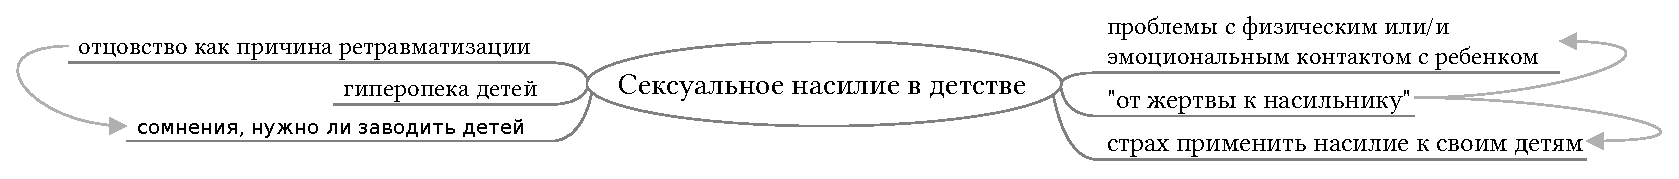
\includegraphics[scale=0.85]{child_sexual_abuse.eps}
  \caption{Child sexual abuse, masculinity and fatherhood}\label{childsexabuse}
 \end{center}

\end{figure}


\subsection*{Сделайте сводную когнитивную карту всех найденных статей}
\begin{figure}[ht!]
 \begin{center}
  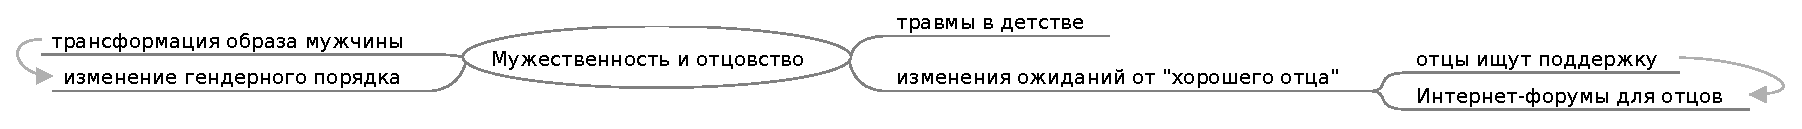
\includegraphics[scale=0.85]{all_articles.eps}
  \caption{Для всех рассмотренных статей}\label{alarticles}
 \end{center}

\end{figure}
\end{landscape}

%\printbibliography[env=gostbibliography,sorting=ntvy]
%\addcontentsline{toc}{chapter}{Литература}

\end{document}
